% This is the Reed College LaTeX thesis template. Most of the work
% for the document class was done by Sam Noble (SN), as well as this
% template. Later comments etc. by Ben Salzberg (BTS). Additional
% restructuring and APA support by Jess Youngberg (JY).
% Your comments and suggestions are more than welcome; please email
% them to cus@reed.edu
%
% See http://web.reed.edu/cis/help/latex.html for help. There are a
% great bunch of help pages there, with notes on
% getting started, bibtex, etc. Go there and read it if you're not
% already familiar with LaTeX.
%
% Any line that starts with a percent symbol is a comment.
% They won't show up in the document, and are useful for notes
% to yourself and explaining commands.
% Commenting also removes a line from the document;
% very handy for troubleshooting problems. -BTS

% As far as I know, this follows the requirements laid out in
% the 2002-2003 Senior Handbook. Ask a librarian to check the
% document before binding. -SN

%%
%% Preamble
%%
% \documentclass{<something>} must begin each LaTeX document
\documentclass[12pt,twoside]{reedthesis}
% Packages are extensions to the basic LaTeX functions. Whatever you
% want to typeset, there is probably a package out there for it.
% Chemistry (chemtex), screenplays, you name it.
% Check out CTAN to see: http://www.ctan.org/
%%
\usepackage{graphicx,latexsym}
\usepackage{amsmath}
\usepackage{amssymb,amsthm}
\usepackage{longtable,booktabs,setspace}
\usepackage{chemarr} %% Useful for one reaction arrow, useless if you're not a chem major
\usepackage[hyphens]{url}
% Added by CII
\usepackage[hidelinks]{hyperref}
\usepackage{lmodern}
\usepackage{float}
\floatplacement{figure}{H}
% End of CII addition
\usepackage{rotating}

% Next line commented out by CII
%%% \usepackage{natbib}
% Comment out the natbib line above and uncomment the following two lines to use the new
% biblatex-chicago style, for Chicago A. Also make some changes at the end where the
% bibliography is included.
%\usepackage{biblatex-chicago}
%\bibliography{thesis}


% Added by CII (Thanks, Hadley!)
% Use ref for internal links
\renewcommand{\hyperref}[2][???]{\autoref{#1}}
\def\chapterautorefname{Chapter}
\def\sectionautorefname{Section}
\def\subsectionautorefname{Subsection}
% End of CII addition

% Added by CII
\usepackage{caption}
\captionsetup{width=5in}
% End of CII addition

% \usepackage{times} % other fonts are available like times, bookman, charter, palatino


% To pass between YAML and LaTeX the dollar signs are added by CII
\title{A Heston implementation}
\author{Fernando O. Teixeira}
% The month and year that you submit your FINAL draft TO THE LIBRARY (May or December)
\date{May 2017}
\division{Applied Mathematics}
\advisor{Advisor F. Name}
%If you have two advisors for some reason, you can use the following
% Uncommented out by CII
% End of CII addition

%%% Remember to use the correct department!
\department{Mathematics}
% if you're writing a thesis in an interdisciplinary major,
% uncomment the line below and change the text as appropriate.
% check the Senior Handbook if unsure.
%\thedivisionof{The Established Interdisciplinary Committee for}
% if you want the approval page to say "Approved for the Committee",
% uncomment the next line
%\approvedforthe{Committee}

% Added by CII
%%% Copied from knitr
%% maxwidth is the original width if it's less than linewidth
%% otherwise use linewidth (to make sure the graphics do not exceed the margin)
\makeatletter
\def\maxwidth{ %
  \ifdim\Gin@nat@width>\linewidth
    \linewidth
  \else
    \Gin@nat@width
  \fi
}
\makeatother

\renewcommand{\contentsname}{Table of Contents}
% End of CII addition

\setlength{\parskip}{0pt}

% Added by CII

\providecommand{\tightlist}{%
  \setlength{\itemsep}{0pt}\setlength{\parskip}{0pt}}

\Acknowledgements{
I want to thank a few people.
}

\Dedication{
You can have a dedication here if you wish.
}

\Preface{
This is an example of a thesis setup to use the reed thesis document
class (for LaTeX) and the R bookdown package, in general.
}

\Abstract{
The preface pretty much says it all. \par  Second paragraph of abstract
starts here.
}

	\bibliographystyle{elsarticle-num}
% End of CII addition
%%
%% End Preamble
%%
%

\usepackage{amsthm}
\newtheorem{theorem}{Theorem}[section]
\newtheorem{lemma}{Lemma}[section]
\theoremstyle{definition}
\newtheorem{definition}{Definition}[section]
\newtheorem{corollary}{Corollary}[section]
\newtheorem{proposition}{Proposition}[section]
\theoremstyle{definition}
\newtheorem{example}{Example}[section]
\theoremstyle{remark}
\newtheorem*{remark}{Remark}
\begin{document}

% Everything below added by CII
      \maketitle
  
  \frontmatter % this stuff will be roman-numbered
  \pagestyle{empty} % this removes page numbers from the frontmatter

      \begin{acknowledgements}
      I want to thank a few people.
    \end{acknowledgements}
  
      \begin{preface}
      This is an example of a thesis setup to use the reed thesis document
      class (for LaTeX) and the R bookdown package, in general.
    \end{preface}
  
      \hypersetup{linkcolor=black}
    \setcounter{tocdepth}{2}
    \tableofcontents
  
      \listoftables
  
      \listoffigures
  
      \begin{abstract}
      The preface pretty much says it all. \par  Second paragraph of abstract
      starts here.
    \end{abstract}
  
      \begin{dedication}
      You can have a dedication here if you wish.
    \end{dedication}
  
  \mainmatter % here the regular arabic numbering starts
  \pagestyle{fancyplain} % turns page numbering back on

  \chapter{Delete line 6 if you only have one
  advisor}\label{delete-line-6-if-you-only-have-one-advisor}
  
  \chapter{Literature Review}\label{lt-review}
  
  This chapter presents the concepts of stochastic calculus, from the
  historic conception of how it first arose through the basic principles
  and applications in finance. More precisely, we address the classical
  Black-Scholes model and its limitations and the Heston model. This model
  is also well known, it introduces the concept of stochastic volatility
  which brings us closer to reality.
  
  \section{Stochastic Calculus}\label{stochastic-calculus}
  
  Stochastic calculus arises from stochastic processes and allows the
  creation of a theory of integration where both the integrand and
  integrator terms are stochastic processes. Stochastic calculus, also
  known as, Itô calculus due to the name of it's creator, the Japanese
  mathematician Kiyosi Itô in the 1940s and 1950s is used for modelling
  financial options and in another wide variety of fields {[}1{]}. In this
  chapter we present the historical contexts in which the tools and models
  used arise, but our focus is introducing the concepts and notations that
  will be further used in our work.
  
  \subsection{Brownian Motion}\label{brownian-motion}
  
  The Brownian motion is the name given to the irregular motion observed
  in the motion of pollen particles suspended in fluid resulting from
  particle collision with atoms or molecules. It is named after Robert
  Brown, the first to have observed the movement in 1828. He noted two
  characteristic in the pollen movement {[}1{]}:
  
  \begin{itemize}
  \item
    the path of a givern particle is very irregular, having a tangent at
    no point
  \item
    the motion of two distinct particles appear to be independent
  \end{itemize}
  
  The first quantitative works in brownian motion come from an interest in
  stock price fluctuation by Bachelier in 1900. Albert Einstein also
  leaned over the subject and in 1905 derived the transition density for
  Brownian motion from molecular-kinectic theory of heat {[}1,2{]}.
  
  In 1923, the Wiener process was coined in honor of Norbert Wiener
  mathematical proof of existence of the brownian motion and stating its
  properties as follows {[}3{]}:
  
  \begin{itemize}
  \item
    \(W_{0}=0\)
  \item
    The change in \(W\), given by \(\Delta W = W_{t+1}-W_{t}\), is
    normally distributed with mean Wero and standard deviation
    \(\sqrt{\Delta t}\), meaning that
    \(\Delta W = \epsilon\sqrt{\Delta t}\), where \(\epsilon\) is
    \(N(0,1)\).
  \item
    If the increment \(\Delta t_1\) does not overlap with the time
    increment \(\Delta t_2\), then \(\Delta W_1\) and \(\Delta W_2\) are
    independent.
  \item
    The process is continuous, meaning that there are no jumps in the
    process.
  \item
    The process is a Markov process. This means that the conditional
    expectation of \(W_{t+1}\) given its entire history is equal to the
    conditional expectation of \(W_{t+1}\) given today's information. This
    can be written as: \(E[W_{t+1}|W_1, ..., W_t] = E[W_{t+1}|W_t]\).
  \item
    Consider the time interval \([0,t]\) with \(n\) equally spaced
    intervals given by \(t_i = \frac{it}{n}\). Then the paths of the
    Brownian motion have unbounded variation, this means that they are not
    differentiable and go towards infinity as \(n\) increases. The
    quadratic variation is given by
    \(\sum_{i=1}^{n}{(Z_{t_i}-Z_{t_{i-1}})^2} \rightarrow t\), meaning
    that when \(n\) increases it stays constant at \(t\).
  \end{itemize}
  
  \subsection{Itô's Lemma}\label{itos-lemma}
  
  Let \(X_{t}\) be a real-valued stochastic process that satisfies
  {[}4--6{]}:
  
  \begin{align}
  X_t = X_0 + \int_{0}^{t} \mu_t dt + \int_{0}^{t} \sigma_t dW_t
  \end{align}
  
  \noindent
  for some \(\mu_t\), \(\sigma_t\) and \(t \in [0,T]\). This equation is
  often rewritten in its differential stochastic form:
  
  \begin{align}
  dX_t = \mu_t dt + \sigma_t dW_t 
  \end{align}
  
  \noindent
  for \(0 \leq t \leq T\).
  
  \subsubsection{Theorem}\label{theorem}
  
  Assume that \(X_t\) has a stochastic differential given by:
  
  \begin{align}
  dX_t = \mu_t dt + \sigma_t dW_t 
  \end{align}
  
  \noindent
  for \(\mu_t\), \(\sigma_t\) and \(t \in [0,T]\). Assume
  \(u: \mathbb{R} \times [0, T] \rightarrow \mathbb{R}\) is continuous and
  that \(\frac{\partial u}{\partial t}\),
  \(\frac{\partial u}{\partial x}\), \(\frac{\partial^2 u}{\partial x^2}\)
  exist and are continuous.
  
  \[ Y_t := u(X_t, t) \] \noindent
  Then Y has the following stochastic differential:
  
  \begin{align} 
  \label{eq:ito}
  \begin{split}
      dY_t &= \frac{\partial u}{\partial t}dt + \frac{\partial u}{\partial x} dX_t + \frac{1}{2}\frac{\partial^2 u}{\partial x^2}\sigma_t^2 dt  \\[10pt] 
      &= \left( \frac{\partial u}{\partial t} + \mu_t \frac{\partial u}{\partial x} + \frac{1}{2}\frac{\partial^2 u}{\partial x^2}\sigma_t^2 \right) dt + \sigma_t \frac{\partial u}{\partial x} dW_t
  \end{split}
  \end{align}
  
  \noindent  where the argument of \(u\),
  \(\frac{\partial u}{\partial x}\) and
  \(\frac{\partial^2 u}{\partial x^2}\) above is \(\left( X_t, t \right)\)
  .
  
  Equation \eqref{eq:ito} is the stochastic equivalent to the chain rule,
  also known as Itô's formula or Itô's chain rule. The proof to this
  theorem is based on the Taylor expansion of the function \(f(X_t, t)\)
  {[}4,5{]}. For practical uses you should write out a second-order Taylor
  expansion for the function to be analyzed and apply the
  \ref{tab:box-calc} multiplication table {[}1{]}.
  
  \begin{longtable}[t]{llr}
  \caption{\label{tab:box-calc}Box calculus}\\
  \toprule
    & $dt$ & $dW_t$\\
  \midrule
  $dt$ & 0 & 0\\
  $dW_t$ & 0 & $dt$\\
  \bottomrule
  \end{longtable}
  
  the \ref{tab:foo2} multiplication table.
  
  \ref{fig:bar}
  
  \begin{Shaded}
  \begin{Highlighting}[]
  \KeywordTok{par}\NormalTok{(}\DataTypeTok{mar =} \KeywordTok{c}\NormalTok{(}\DecValTok{4}\NormalTok{, }\DecValTok{4}\NormalTok{, }\FloatTok{0.1}\NormalTok{, }\FloatTok{0.1}\NormalTok{))}
  \KeywordTok{plot}\NormalTok{(pressure, }\DataTypeTok{pch =} \DecValTok{19}\NormalTok{, }\DataTypeTok{type =} \StringTok{"b"}\NormalTok{)}
  \end{Highlighting}
  \end{Shaded}
  
  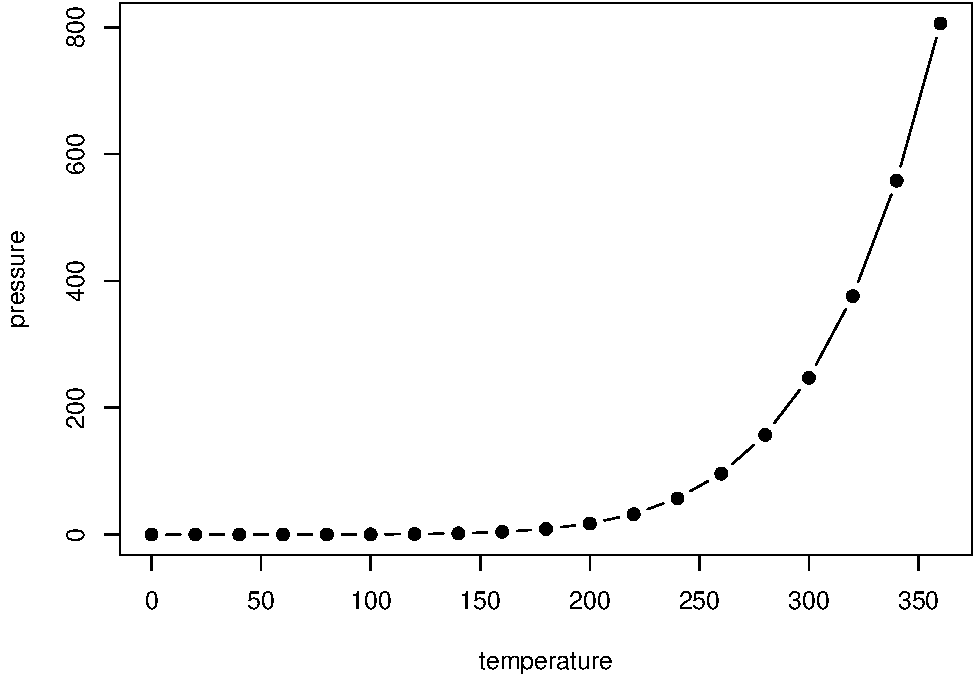
\includegraphics{thesis_files/figure-latex/bar-1.pdf}
  
  \section{Black-Scholes Model}\label{black-scholes-model}
  
  \begin{itemize}
  \tightlist
  \item
    Model
  \end{itemize}
  
  \subsection{Derivative Contracts}\label{derivative-contracts}
  
  European Call and Put
  
  \subsection{Limitations}\label{limitations}
  
  \section{Heston Model}\label{heston-model}
  
  \chapter{Mathematics and Science}\label{math-sci}
  
  \chapter{This chunk ensures that the thesisdown package
  is}\label{this-chunk-ensures-that-the-thesisdown-package-is}
  
  \chapter*{Conclusion}\label{conclusion}
  \addcontentsline{toc}{chapter}{Conclusion}
  
  \chapter{The First Appendix}\label{the-first-appendix}
  
  \chapter*{References}\label{references}
  \addcontentsline{toc}{chapter}{References}
  
  \hypertarget{refs}{}
  \hypertarget{ref-ubbo}{}
  {[}1{]} U.F. Wiersema, Brownian motion calculus, John Wiley \& Sons,
  2008.
  
  \hypertarget{ref-karatzas2012brownian}{}
  {[}2{]} I. Karatzas, S. Shreve, Brownian motion and stochastic calculus,
  Springer Science \& Business Media, 2012.
  
  \hypertarget{ref-helgadottir2016option}{}
  {[}3{]} A.D. Helgadóttir, L. Ionescu, Option pricing within the heston
  model, (2016).
  
  \hypertarget{ref-tong2012option}{}
  {[}4{]} Z. Tong, Option pricing with long memory stochastic volatility
  models, PhD thesis, Université d'Ottawa/University of Ottawa, 2012.
  
  \hypertarget{ref-evans2012introduction}{}
  {[}5{]} L.C. Evans, An introduction to stochastic differential
  equations, American Mathematical Soc., 2012.
  
  \hypertarget{ref-steele2012stochastic}{}
  {[}6{]} J.M. Steele, Stochastic calculus and financial applications,
  Springer Science \& Business Media, 2012.


  % Index?

\end{document}

